\documentclass[11pt, dvipsnames, DIV=12]{scrreprt}
\usepackage{babel}

\usepackage[utf8]{inputenc}
\usepackage[T1]{fontenc}
\usepackage{natbib}
\bibliographystyle{abbrvnat}
\usepackage{subcaption}
\usepackage{booktabs}
\usepackage{multirow}
\usepackage{url}
\usepackage{tikz}
\usepackage{paralist}

\usepackage{ifthen}
\newcommand{\CC}[1][]{$\text{C\hspace{-.25ex}}^{_{_{_{++}}}}
\ifthenelse{\equal{#1}{}}{}{\text{\hspace{-.625ex}#1}}$}

\usepackage{bm}
\usepackage{amsmath}
\usepackage{amssymb}
\usepackage{amsthm}
\usepackage{amsfonts}
\usepackage{thmtools}		
\usepackage{mleftright}
\usepackage{stmaryrd}
\usepackage{nicefrac}
\usepackage{algorithm}
\usepackage{algorithmicx}
\usepackage[noend]{algpseudocode}
\renewcommand{\algorithmicrequire}{\textbf{Input:}}
\renewcommand{\algorithmicensure}{\textbf{Output:}}

\usepackage{bbold} % For the indicator function: \mathbb{1}


% Fixes some spacing issues with braces.
\let\originalleft\left
\let\originalright\right
\renewcommand{\left}{\mathopen{}\mathclose\bgroup\originalleft}
\renewcommand{\right}{\aftergroup\egroup\originalright}

\theoremstyle{definition}
\newtheorem{theorem}{Theorem}
\newtheorem{conjecture}{Conjecture}
\newtheorem{proposition}[theorem]{Proposition}
\newtheorem{insight}{Insight}
\newtheorem{observation}{Observation}
\newtheorem{lemma}[theorem]{Lemma}
\newtheorem{corollary}[theorem]{Corollary}
\newtheorem{definition}[theorem]{Definition}
\newtheorem{example}[theorem]{Example}
\newtheorem{remark}[theorem]{Remark}
\newtheorem{claim}[theorem]{Claim}
\newtheorem{fact}[theorem]{Fact}
\usepackage{thm-restate}
\usepackage[mathic=true]{mathtools}
\usepackage{fixmath}
\usepackage{siunitx}

\usepackage{pifont}
\newcommand{\cmark}{\ding{51}}
\newcommand{\xmark}{\ding{55}}
\usepackage{blindtext}

\usepackage{todonotes}

\usepackage{enumitem}
\setlist[enumerate]{itemsep=0.2ex, topsep=0.5\topsep}
\setlist[description]{itemsep=0.2ex, topsep=0.5\topsep}
\setlist[itemize]{itemsep=0.2ex, topsep=0.5\topsep}


% Let cleveref and thmtools work together
\makeatletter
\def\thmt@refnamewithcomma #1#2#3,#4,#5\@nil{%
\@xa\def\csname\thmt@envname #1utorefname\endcsname{#3}%
\ifcsname #2refname\endcsname
\csname #2refname\expandafter\endcsname\expandafter{\thmt@envname}{#3}{#4}%
\fi
}
\makeatother

% Removed 'pagebackref,' as it makes the bilbipgraphy more cluddered in my opinion
\usepackage[
pdfa,
hidelinks,
pdftex, 
pdfdisplaydoctitle,
pdfpagelabels,
pdfauthor={},
pdftitle={},
pdfsubject={},
pdfkeywords={},
pdfproducer={Latex with the hyperref package},
pdfcreator={pdflatex}
]{hyperref}

\usepackage[capitalise,noabbrev]{cleveref}   

\usepackage{microtype}
\usepackage{ellipsis}

\usepackage[scaled=0.86]{helvet}
\usepackage{lmodern}

\usepackage{pgfplots}


% Bold. 
\newcommand{\mF}{\mathbf{F}}
\newcommand{\mG}{\mathbf{G}}
\newcommand{\mH}{\mathbf{H}}
\newcommand{\mL}{\mathbf{L}}
\newcommand{\mI}{\mathbf{I}}

\newcommand{\mW}{\mathbf{W}}
\newcommand{\ma}{\mathbf{a}}
\newcommand{\mb}{\mathbf{b}}
\newcommand{\mw}{\mathbf{w}}

\newcommand{\ba}{\ensuremath{{\bf a}}}
\newcommand{\bb}{\ensuremath{{\bf b}}}
\newcommand{\bc}{\ensuremath{{\bf c}}}

% Calligraphic.
\newcommand{\cA}{\mathcal{A}}
\newcommand{\cB}{\mathcal{B}}
\newcommand{\cC}{\mathcal{C}}
\newcommand{\cF}{\mathcal{F}}
\newcommand{\cG}{\mathcal{G}}
\newcommand{\cH}{\mathcal{H}}
\newcommand{\cN}{\mathcal{N}}
\newcommand{\cO}{\mathcal{O}}
\newcommand{\cP}{\mathcal{P}}
\newcommand{\cR}{\mathcal{R}}
\newcommand{\cS}{\mathcal{S}}
\newcommand{\cT}{\mathcal{T}}
\newcommand{\cU}{\mathcal{U}}
\newcommand{\cV}{\mathcal{V}}
\newcommand{\cX}{\mathcal{X}}


% Sans serif.
\newcommand{\sC}{\mathsf{C}}

% Blackboard.
\newcommand{\Fb}{\mathbb{F}}
\newcommand{\Gb}{\mathbb{G}}
\newcommand{\Nb}{\mathbb{N}}
\newcommand{\Qb}{\mathbb{Q}}
\newcommand{\Rb}{\mathbb{R}}
\newcommand{\Zb}{\mathbb{Z}}

% Multiset Definition
\newcommand{\MSopen}{\{\!\!\{}
\newcommand{\MSclose}{\}\!\!\}}

% 1-WL+NN
\newcommand{\wlnn}{\text{1-WL+NN}}
\newcommand{\wliso}{\simeq_{\text{1WL}}}
\newcommand{\xnn}{\mathcal{X}^{n \times n}}
\newcommand{\gapp}{\text{GNN-Approximating}}
\newcommand{\wldisc}{\text{1-\!WL-Discriminating}}
\newcommand{\wl}{\text{1-\!WL}}
\newcommand{\mlp}{\text{MLP}}


\usetikzlibrary{calc}


\usepackage[auth-lg]{authblk}
\newcommand{\cm}[1]{{{\textcolor{purple}{\textbf{[CM:} {#1}\textbf{]}}}}}


\renewcommand*{\Affilfont}{\large\normalfont}
\renewcommand*{\Authfont}{\normalfont}

\recalctypearea
\setcounter{Maxaffil}{2}

\title{\emph{A Theoretical and Empirical Investigation into the Equivalence of Graph Neural Networks and the Weisfeiler-Leman Algorithm}\\
\vspace{20pt}\small{\normalfont From the faculty of Mathematics, Physics, and Computer Science for the purpose of obtaining the academic degree of Bachelor of Sciences.}
}
\author{\textbf{Eric Tillmann Bill}}
\affil{\vspace{100pt}}

\author{Supervision:\\Prof. Dr. rer. nat. Christopher Morris}
\affil{Informatik 6\\RWTH Aachen University}

\date{\vspace{-30pt}}

\renewcommand{\thesection}{\arabic{section}}

\begin{document}

\maketitle
\tableofcontents
\newpage



\section{Definition}
\begin{definition}[1-WL Relation]
    For any graphs $G,H$ we will denote $G \wliso H$ if the 1-WL isomorphism test can not distinguish both graphs. Note that due to the soundness of this algorithm, if $G \not\wliso H$, we always can conclude that $G \not\simeq H$.
\end{definition}

\begin{definition}
    Let $f: \xnn \rightarrow A^K$ be a well-defined encoding function compatible with the $\wlnn$ framework and $R$ an arbitrary domain. Then we call $\cC$ a collection of permutation invariant functions from $\xnn$ to $R$ that are computed by $\wlnn$, where for every MLP working over $A^K$ to $R$ there exists $\beta \in \cC$ with: $\beta: \xnn \rightarrow R, G \mapsto \text{MLP} \circ f(G)$.
\end{definition}

\begin{definition}
    Let $\mathcal{C}$ be a collection of permutation invariant functions from $\mathcal{X}^{n\times n}$ to $\Rb$. We say $\mathcal{C}$ is \textbf{\wldisc} if for all graphs $G_1, G_2 \in \mathcal{X}$ for which the 1-WL isomorphism test concludes non-isomorphic, there exists a function $h \in \mathcal{C}$ such that $f(G_1) \neq f(G_2)$.
\end{definition}

\begin{definition}
    Let $\mathcal{C}$ be a collection of permutation invariant functions from $\mathcal{X}^{n\times n}$ to $\Rb$. We say $\mathcal{C}$ is \textbf{\gapp} if for all permutation-invariant functions $\mathcal{A}$ computed by a GNN, and for all $\epsilon \in \Rb$ with $\epsilon > 0$, there exists $h_{\cA,\epsilon} \in \mathcal{C}$ such that $\| \cA - h_{\cA,\epsilon} \|_\infty := \sup_{G \in \mathcal{X}} |f(G) - h_{\cA,\epsilon}(G)| < \epsilon$
\end{definition}

\section{Theorems}
In this thesis we concentrate on finite graphs. We therefore, let $\mathcal{X}$ be a XYS.

\begin{theorem}[$\wlnn \subseteq \text{GNN}$]\label{theorem:1wl_in_gnn}
    Let $\cC$ be a collection of functions from $\cX$ to $\Rb$ computed by $\wlnn$ and $\cX$ finite set of graphs. If $\cC$ is $\wldisc$, then there exists an augmentation $\cC'$ of $\cC$ that is computable by $\wlnn$, such that for every function $\cA$ computed by a GNN, $\cA \in \cC'$.
\end{theorem}
\noindent With this theorem we can conclude that every function computable by a GNN is also computable by a $\wlnn$.


\section{Proofs}
Throughout this thesis we will concentrate on finite graphs, such that we let $\mathcal{X}$ be $\mathcal{X} := \{1, \dots, k\}$ for an arbitrary $k \in \Nb$. We will prove \cref{theorem:1wl_in_gnn} by introducing a couple of small lemmas, which combined prove the theorem. In detail, in \cref{lem:wl_disc_exists} we show the existence of collections computed by $\wlnn$ that are 1-\!WL-Discriminating. In \cref{lem:wlnn_permutation_invariance,lem:wl_relation_equivalence,lem:composition_lemma} we derive properties of $\wlnn$ functions we will use throughout \cref{lem:encoding-indicator-func1,lem:encoding-indicator-func2,lem:decompose_gnn_as_wl} with which we prove the theorem.
We took great inspiration for \cref{lem:encoding-indicator-func1,lem:encoding-indicator-func2,lem:decompose_gnn_as_wl} from the proof presented in section 3.1 in the work of \cite{Chen2019}.

\begin{lemma}\label{lem:wl_disc_exists}
    There exists a collection $\cC$ of functions from $\cX$ to $\Rb$ computed by $\wlnn$ that is 1-\!WL-Discriminating.
\end{lemma}
\begin{proof}
We consider the collection $\mathfrak{B}_k$ of functions computed by \wlnn, where every $\mathcal{B} \in \mathfrak{B}_k$ is of the form $\mathcal{B}(\cdot) = \text{MLP} \circ f_{\text{enc}}(\cdot)$. Here MLP is an arbitrary multilayer perceptron mapping vectors from $\Nb^K$ to $\Rb$ and $f$ the \textit{counting-encoding} function. Further, let $G_1, G_2 \in \mathcal{X}^{n\times n}$ such that the 1-WL isomorphism test concludes non-isomorphic ($G_1 \not\simeq G_2$). We denote with $(C_{\infty})_G$ the final coloring computed by the 1-WL algorithm when applied on $G$.
Due to the 1-WL isomorphism test concluding $G_1 \not\simeq G_2$, there exists a color $c \in \Nb$ such that $(C_{\infty})_{G_1}(c) \neq (C_{\infty})_{G_2}(c)$. If we now consider as MLP the following function $\text{MLP}: \Nb^K \rightarrow \Rb, v \mapsto W \cdot v$ with $W \in \Nb^{1 \times K}$ such that $W_{1,c} := 1$ and $W_{1,i} := 0$ for all $i \in [K] \setminus \{c\}$. Then we can conclude that $\mathcal{B}(G_1) \neq \mathcal{B}(G_2)$. Since $G_1,G_2$ are arbitrary, we can conclude the proof.
\end{proof}

\begin{lemma}[$\wlnn$ Permuation Invariance]\label{lem:wlnn_permutation_invariance}
    Let $\cC$ be a collection of functions computed by $\wlnn$, then every function $\cB \in \cC$ is permutation-invariant.
\end{lemma}

\begin{proof}
    Let $\cC$ be a collection of functions computed by $\wlnn$. Let $\cB$ be an arbitrary function in $\cC$, then $\cB$ is comprised as follows: $\cB(\cdot) = \text{MLP} \circ f_{\text{enc}} \circ \wl(\cdot)$. Since, the $\wl$ coloring algorithm is permutation-invariant, the overall function is permutation invariant.
\end{proof}

\begin{lemma}[$\wlnn$ Equivariance]\label{lem:wl_relation_equivalence}
    Let $\cC$ be a collection of functions computed by $\wlnn$, then for every function $\cB \in \cC$ and every pair of graphs $G_1, G_2 \in \xnn:$ if $G_1 \wliso G_2$ than $\cB(G_1) = \cB(G_2)$.
\end{lemma}

\begin{proof}
    Let $\cC$ be a collection of functions computed by $\wlnn$. Let $\cB$ be an arbitrary function in $\cC$, then $\cB$ is comprised as follows: $\cB(\cdot) = \text{MLP} \circ f_{\text{enc}} \circ \wl(\cdot)$. Let $G_1, G_2 \in \xnn$ be arbitrary graphs with $G_1 \wliso G_2$, then by definition of the relation $\wliso$ we know that $\wl(G_1) = \wl(G_2)$. With this the equivalence follows immediatly.
\end{proof}

\begin{lemma}[Composition Lemma]\label[lemma]{lem:composition_lemma}
    Let $\cC$ be a collection of functions computed by $\wlnn$. Further, $h_1, \dots h_n \in \cC$ and $\text{MLP}$ a multilayer perceptron, than the function $\cA$ composed of $\cA(\cdot) := \text{MLP}(h_1(\cdot), \ldots, h_n(\cdot))$ is also computable by $\wlnn$.
\end{lemma}
\begin{proof}
    Assume the above and let $f_{1}, \ldots, f_{n}$ be the encoding functions, as well as $\text{MLP}_1, \ldots, \text{MLP}_n$ be the multilayer perceptrons used by $h_1, \dots h_n$ respectively. The idea of this proof is, we construct an encoding function $f^*$ that maps a coloring $C_\infty$ to a concatenation of the vectors obtained when applying each encoding function $f_i$ individually. Additionally, we construct a multilayer perceptron $\mlp^*$ that takes in this concatenation of vectors and simulates all $\text{MLP}_1, \ldots, \text{MLP}_n$ simultaneously on their respective section of the encoding vector of $f^*$, and applies afterwards the new $\mlp$ on the concatenation of the output of all $\mlp_i$.  See \autoref{fig:proof_idea_parallelism} for a sketch of the proof idea. A complete proof can be found in the Appendix, as this proof is very technical and not that interesting.

    \begin{figure}[H]
        \centering
        \begin{tikzpicture}

    \tikzset{line/.style={draw,thick}}
    \tikzset{arrow/.style={line,->,>=stealth}}
    \tikzset{node/.style={circle,inner sep=0pt,minimum width=15pt}}
    
    \node (inputG) {$G$};
    \node (coloring) [right =of inputG] {$M_G$};
    \node (firstV) [right =of coloring] {$\begin{bmatrix*}
        f_1(M_G)\\
        \vdots\\
        f_n(M_G)
    \end{bmatrix*}$};
    \node (inp1) [above right =of firstV] {$f_1(M_G)$};
    \node (inp2) [below right =of firstV] {$f_n(M_G)$};
    \node (out1) [right =of inp1] {$o_1$};
    \node (out2) [right =of inp2] {$o_n$};
    \node (out) [below right =of out1, above right =of out2] {$\begin{bmatrix*}
        o_1\\
        \vdots\\
        o_n
    \end{bmatrix*}$};
    \node (dot1) [right =of firstV] {$\vdots$};
    \node (final_out) [right =of out] {$O$};
    \node (dot2) [below =of out1] {$\vdots$};

    

    \draw[|-latex] (inputG.east) to node[text width=2.5cm,midway,above,align=center] {$\wl$} (coloring.west);

    \draw[-latex] (coloring.east) to node[text width=2.5cm,midway,above,align=center] {$f^*$} (firstV.west);

    \draw[-latex] (firstV.east) -- (inp1.west);

    \draw[-latex] (firstV.east) -- (inp2.west);

    \draw[|-latex] (inp1.east) to node[text width=2.5cm,midway,above,align=center] {$\text{MLP}_1$} (out1.west);

    \draw[|-latex] (inp2.east) to node[text width=2.5cm,midway,above,align=center] {$\text{MLP}_n$} (out2.west);

    \draw[-latex] (out1.east) -- (out.west);
    \draw[-latex] (out2.east) -- (out.west);

    \draw[|-latex] (out.east) to node[text width=2.5cm,midway,above,align=center] {$\mlp^\bullet$} (final_out.west);

    %\draw [thick, decoration={brace,mirror,raise=0.5cm},decorate, below =of out2] (firstV.south) -- (final_out.west);


    %\draw (-1.5,0.75) node {$\cA(G):$};
    %\draw (-1.0, 0.0) node {$G$};

    %\draw [|-latex] (-0.6,0) -- node [text width=2.5cm,midway,above,align=center ] {1-WL} (1.0,0);

    %\draw (1.6, 0.0) node {$(M_G)_G$};

    %\draw [|-latex] (2.4, 0.0) -- node [text width=2.5cm,midway,above,align=center ] {$f$} (3.25, 0.0);
    
    %\draw (3.5, 0.0) node {$v$};

    %\draw (5.0, 1.0) node {$v$};
    %\draw (5.0, -1.0) node {$v$};
    
\end{tikzpicture}
        \caption{Sketch of the proof we use to prove lemma XYZ.}
        \label{fig:proof_idea_parallelism}
    \end{figure}
\end{proof}
    


\begin{lemma}\label[lemma]{lem:encoding-indicator-func1}
    Let $\cC$ be a collection of functions from $\xnn$ to $\Rb$ computed by $\wlnn$ that is $\wldisc$. Then for all $G \in \xnn$, there exists a function $h_G$ computable by $\wlnn$ such that for all $G^* \in \xnn: h_G(G^*) = 0$ if and only if $G \wliso G^*$.
\end{lemma}

\begin{proof}
    For any $G_1, G_2 \in \xnn$ with $G_1 \not\wliso G_2$ let $f_{G_1, G_2} \in \cC$ be the function distinguishing them, with $f_{G_1, G_2}(G_1) \neq f_{G_1, G_2}(G_2)$. We define the function $\overline{f}_{G_1}$ working over $\xnn$ as follows:
    \begin{align}\label{eq:lem:encoding-indicator-func2}
        \overline{f}_{G_1, G_2}(\cdot) &= |f_{G_1, G_2}(\cdot) - f_{G_1, G_2}(G_1)| \nonumber \nonumber\\
        &= \max(f_{G_1, G_2}(\cdot) - f_{G_1, G_2}(G_1)) + \max(f_{G_1, G_2}(G_1) - f_{G_1, G_2}(\cdot))
    \end{align}
    Note, that in the formula above ``$h_{G_1, G_2}(G_1)$'' is a fixed constant and the resulting function $\overline{f}_{G_1, G_2}$ is non-negative.
    Let $G_1 \in \xnn$ now be fixed, we will construct the function $h_G$ with the desired properties as follows:
    \begin{align*}
        h_{G_1}(x) = \sum_{G_2 \in \xnn, \ G_1 \not\wliso G_2} \overline{f}_{G_1, G_2}(x).
    \end{align*}
    Since $\cX$ is finite, the sum is finite and therefore well-defined. Next, we will prove that for a fixed graph $G_1 \in \xnn$, the function $h_{G_1}$ is correct on input $G^* \in \xnn$:
    \begin{enumerate}
        \item If $G_1 \wliso G^*$, then for every function $\overline{f}_{G_1, G_2}$ of the sum with $G_1 \not\wliso G_2$, we know, using \cref{lem:wl_relation_equivalence}, that $\overline{f}_{G_1, G_2}(G^*)$ is equal to $f_{G_1, G_2}(G_1)$ which is by definition $0$, such that $h_{G_1}(G^*) = 0$.
        \item If $G_1 \not\wliso G^*$, then $\overline{f}_{G_1, G^*}(G^*)$ is a summand of the overall sum, and since $\overline{f}_{G_1, G^*}(G^*) > 0$, than due to the non-negativity of each function $\overline{f}$ we can conclude $h_{G_1}(G*) > 0$.
    \end{enumerate}

    This function can be encoded in an MLP by replacing the $\max$ terms of the last line in \autoref{eq:lem:encoding-indicator-func2} by the activation function ReLU. Therefore, we can conclude with \cref{lem:composition_lemma} that for every graph $G$, $h_G$ is also $\wlnn$ computable.
\end{proof}

\begin{lemma}\label[lemma]{lem:encoding-indicator-func2}
    Let $\mathcal{C}$ be a collection of functions from $\mathcal{X}^{n \times n}$ to $\Rb$ computed by $\wlnn$ so that for all $G \in \mathcal{X}^{n \times n}$, there exists $h_G \in \mathcal{C}$ satisfying $h_G(G^*) = 0 $ if and only if $G \wliso G^*$ for all $G^* \in \mathcal{X}^{n \times n}$. Then for every $G \in \xnn$, there exists a function $\varphi_G $ computable by $\wlnn$ such that for all $G^* \in \xnn$: $\varphi_G(G^*) = \mathbb{1}_{G \wliso G^*}$.
\end{lemma}
\begin{proof}
    Assuming the above. Due to $\cX$ being finite, we can define for every graph $G$ the constant:
    \begin{equation*}
        \delta_G := \frac{1}{2} \min_{G^* \in \xnn , G \not\wliso G^*} |h_G(G^*)| > 0.
    \end{equation*}
    With this constant, we can use a so-called ``bump'' function working from $\Rb$ to $\Rb$ that will be similar to the indicator function. We define this function for parameter $a \in \Rb$ with $a > 0$ as:
    \begin{equation*}
        \psi_a(x) := \max(\frac{x}{a} -1,\ 0) + \max(\frac{x}{a}+1, \ 0) - 2 \cdot \max(\frac{x}{a}, \ 0).
    \end{equation*}
    The interesting property of $\psi_a$ is that it maps every value $x$ to $0$, except when $x$ is being drawn from the interval $(-a, a)$. In particular, it maps $x$ to $1$ if and only if $x$ is equal to $0$. See \autoref{fig:bump_function} in the Appendix for a plot of the relevant part of this function with exemplary values for $a$.
    
    We use these properties to define for every graph $G \in \xnn$ the function $\varphi_G(G^*) := \psi_{\delta_G} (h_G(G^*))$. 
    We will quickly demonstrate that this function is equal to the indicator function, for this let $G$ be fixed and $G^*$, an arbitrary graph from $\xnn$, the input:
    \begin{enumerate}
        \item If $G \wliso G^*$, then $h_G(G^*) = 0$ resulting in $\varphi_G(G^*) = \psi_{\delta_G}(0) = 1$.
        \item If $G \not\wliso G^*$ then $h_G(G^*) > 0$, such that $|h_G(G^*)|> \delta_G$ resulting in $\varphi_G(G^*) = 0$.
    \end{enumerate}
    Note we can encode each $\varphi_G$ via a single MLP layer, where $\delta_G$ is a constant and the $\max$ operator is replaced by the non-linear activation function ReLU of the layer. With \cref{lem:composition_lemma} we can therefore conclude that $\varphi_G$ is computable by $\wlnn$ for every graph $G \in \xnn$.
\end{proof}

\begin{lemma}\label{lem:decompose_gnn_as_wl}
    Let $\mathcal{C}$ be a collection of functions from $\mathcal{X}^{n \times n}$ to $\Rb$ computed by $\wlnn$ so that for all $G \in \mathcal{X}^{n \times n}$, there exists 
    $\varphi_G \in \cC$ satisfying $\forall G^* \in \xnn: \varphi_G(G^*) = \mathbb{1}_{G \wliso G^*}$, then $C$ is also \gapp.
\end{lemma}

\begin{proof}
    Assume the above. For any permutation invariant function $\mathcal{A}$ computed by an GNN that works over $\xnn$ to $\Rb$, we show that it can be decomposed it as follows for any $G^* \in \mathcal{X}^{n \times n}$:
    \begin{align}
        \mathcal{A}(G^*) &= \Bigl( \ \frac{1}{|\xnn/\!{\wliso}(G^*)|}\sum_{G \in \xnn} \mathbb{1}_{G^* \wliso G} \Bigr) \cdot \mathcal{A}(G^*) \nonumber \\
        &= \frac{1}{|\xnn/\!{\wliso}(G^*)|}\sum_{G \in \mathcal{X}^{n \times n}} \mathcal{A}(G) \cdot \mathbb{1}_{G^* \wliso G} \nonumber \\
        &= \sum_{G \in \mathcal{X}^{n \times n}} \frac{\mathcal{A}(G)}{|\xnn/\!{\wliso}(G)|}  \cdot \varphi_G(G^*)
    \end{align}
    with $\xnn/\!{\wliso}(G^*)$ denoting the set of all graphs $G$ over $\xnn$ that are equivalent to $G^*$ according to the $\wliso$ relation.

    Since $\cA$ is permutation-invariant, and GNNs are at most as good as the 1-WL algorithm in distinguishing non-isomorphic graphs, we can use the fact that for every graph $G,H \in \xnn$ with $G \wliso H$: $\cA(G) = \cA(H)$. Therefore, we can decompose $\cA$ as outlined above. We can encode this decomposition in a single MLP layer with $\frac{\cA(G)}{|\xnn/\!{\wliso}(G)|}$ being a constant and $\varphi_G \in \cC$ encoding the indicator function. Combined with the \cref{lem:composition_lemma}, we can conclude that $\cA$ is computable by $\wlnn$. Important to note, we can only do this since $\cX$ is finite, making the overall sum finite and the size of $\xnn/\!{\wliso}(G)$ well-defined for all graphs.
    
\end{proof}


\newpage
\section*{Appendix}
\subsection*{Figures and graphs}
\begin{figure}[H]
    \centering
    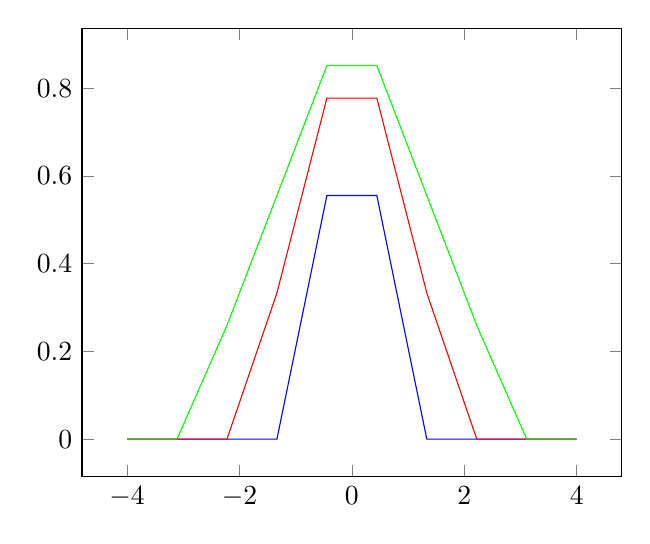
\begin{tikzpicture}
    \begin{axis}
    \addplot[domain=-4:4, samples=10, color=blue,]{max(x-1,0) + max(x+1,0) - 2*max(x,0)};
    \addplot[domain=-4:4, samples=10, color=red,]{max(x/2-1,0) + max(x/2+1,0) - 2*max(x/2,0)};
    \addplot[domain=-4:4, samples=10, color=green,]{max(x/3-1,0) + max(x/3+1,0) - 2*max(x/3,0)};
    \end{axis}
\end{tikzpicture}
    \caption{Illustration of the so-called ``bump'' function $\psi_a(x)$ with $a = 1$ in blue, $ a = 2$ in red and $a = 3$ in green.}
    \label{fig:bump_function}
\end{figure}

\subsection*{Proofs}
\begin{proof}[\cref{lem:composition_lemma}]
    Let $\cC$ be a collection of functions computed by $\wlnn$, $h_1, \dots h_n \in \cC$, and $\text{MLP}$ a multilayer perceptron. Further, let $f_{1}, \ldots, f_{n}$ be the encoding functions, as well as $\text{MLP}_1, \ldots, \text{MLP}_n$ be the multilayer perceptrons used by $h_1, \dots h_n$ respectively. As outlined above, we will now construct $f^*$ and $\mlp^*$.

    We define the new encoding function $f^*$ to work as follows on coloring $C_\infty$:
    \begin{equation*}
        f^*(C_\infty) := \textsf{concat}(f_1(C_\infty), \ldots, f_n(C_\infty)),
    \end{equation*}
    where $\textsf{conccat}$ is the concatenation functions, concatenating all encoding vectors to one single vector.
\end{proof}



\setcitestyle{numbers}
\bibliography{references}
\end{document}